\documentclass{article}
\usepackage[utf8]{inputenc}
\usepackage[papersize={8.5in,11in},margin=0.8in]{geometry}
\usepackage{xcolor}
\usepackage{color, colortbl}
\usepackage{graphicx}
\usepackage{tikz}
\usepackage{amssymb}
\usepackage{amsmath}
\usetikzlibrary{positioning}
\usetikzlibrary{graphs,graphs.standard}


\title{CS520 Written HW 1}
\author{John Caruthers}
\date\today

\begin{document}
\maketitle

\begin{itemize}
    \item[1] Assume we have a hash table with 9 entries, and the hash function: $x\bmod{9}$.
    \begin{itemize}
        \item[a)] Show the entries in the hash table after 1, 4, 8, 14, 22, 9 are inserted. Assume \textbf{separate chaining}.
        \begin{align}
            1\bmod{9}&=1\nonumber\\
            4\bmod{9}&=4\nonumber\\
            8\bmod{9}&=8\nonumber\\
            14\bmod{9}&=5\nonumber\\
            22\bmod{9}&=4\nonumber\\
            9\bmod{9}&=0\nonumber
        \end{align}

        Hash table representation using hash(x)$=x\bmod{9}$, and separate chaining for collision resolution:
        
        \begin{center}
            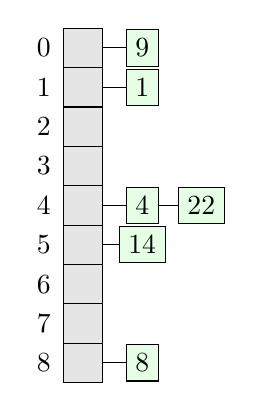
\begin{tikzpicture}
               [dot/.style = {minimum size = 0.5cm, draw, fill=gray!20}, dot1/.style={minimum size = 0.3cm, draw, fill=green!10}]
                % Index in has table
                \node  (0) at (-0.5,0) {$0$};
                \node  (1) at (-0.5,-0.5) {$1$};
                \node  (2) at (-0.5,-1) {$2$};
                \node  (3) at (-0.5,-1.5) {$3$};
                \node  (4) at (-0.5,-2) {$4$};
                \node  (5) at (-0.5,-2.5) {$5$};
                \node  (6) at (-0.5,-3) {$6$};
                \node  (7) at (-0.5,-3.5) {$7$};
                \node  (8) at (-0.5,-4) {$8$};
                % Nodes representing spots in memory at corresponding index
                \node[dot] (a) at (0, 0) {};
                \node[dot] (b) at (0,-0.5) {};
                \node[dot] (c) at (0,-1) {};
                \node[dot] (d) at (0,-1.5) {};
                \node[dot] (e) at (0,-2) {};
                \node[dot] (f) at (0,-2.5) {};
                \node[dot] (g) at (0,-3) {};
                \node[dot] (h) at (0,-3.5) {};
                \node[dot] (i) at (0,-4) {};
                % Chains
                \node[dot1] (a9) at (0.75,0) {$9$};
                \node[dot1] (b1) at (0.75,-0.5) {$1$};
                \node[dot1] (e4) at (0.75,-2) {$4$};
                \node[dot1] (e22) at (1.5,-2) {$22$};
                \node[dot1] (f14) at (0.75,-2.5) {$14$};
                \node[dot1] (i8) at (0.75,-4) {$8$};
                % Lines
                \path[-] (a) edge (a9);
                \path[-] (b) edge (b1);
                \path[-] (e) edge (e4);
                \path[-] (e4) edge (e22);
                \path[-] (f) edge (f14);
                \path[-] (i) edge (i8);
            \end{tikzpicture}
        \end{center}
        
        \item[b)] Show the entries in the hash table after 1, 4, 8, 14, 22, 9 are inserted. Assume \textbf{linear probing}.

        \begin{center}
            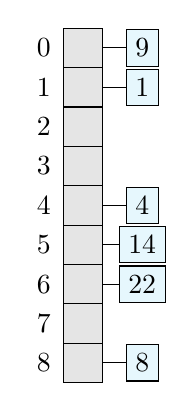
\begin{tikzpicture}
                [dot/.style = {minimum size = 0.5cm, draw, fill=gray!20}, dot1/.style={minimum size = 0.3cm, draw, fill=cyan!10}]
                % Index in has table
                \node  (0) at (-0.5,0) {$0$};
                \node  (1) at (-0.5,-0.5) {$1$};
                \node  (2) at (-0.5,-1) {$2$};
                \node  (3) at (-0.5,-1.5) {$3$};
                \node  (4) at (-0.5,-2) {$4$};
                \node  (5) at (-0.5,-2.5) {$5$};
                \node  (6) at (-0.5,-3) {$6$};
                \node  (7) at (-0.5,-3.5) {$7$};
                \node  (8) at (-0.5,-4) {$8$};
                % Nodes representing spots in memory at corresponding index
                \node[dot] (a) at (0, 0) {};
                \node[dot] (b) at (0,-0.5) {};
                \node[dot] (c) at (0,-1) {};
                \node[dot] (d) at (0,-1.5) {};
                \node[dot] (e) at (0,-2) {};
                \node[dot] (f) at (0,-2.5) {};
                \node[dot] (g) at (0,-3) {};
                \node[dot] (h) at (0,-3.5) {};
                \node[dot] (i) at (0,-4) {};
                % linear probes
                \node[dot1] (a9) at (0.75,0) {$9$};
                \node[dot1] (b1) at (0.75,-0.5) {$1$};
                \node[dot1] (e4) at (0.75,-2) {$4$};
                \node[dot1] (g22) at (0.75,-3) {$22$};
                \node[dot1] (f14) at (0.75,-2.5) {$14$};
                \node[dot1] (i8) at (0.75,-4) {$8$};
                % Lines
                \path[-] (a) edge (a9);
                \path[-] (b) edge (b1);
                \path[-] (e) edge (e4);
                \path[-] (g) edge (g22);
                \path[-] (f) edge (f14);
                \path[-] (i) edge (i8);
            \end{tikzpicture}
        \end{center}

        \newpage
        
        \item[c)] Assume \textbf{linear probing} is used. Suppose now 10 is inserted. Now for the following searches, show the result of the search and how many entries need to be examined before the search return the result?
        \begin{center}
            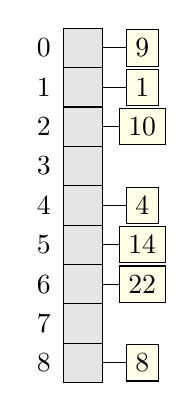
\begin{tikzpicture}
                [dot/.style = {minimum size = 0.5cm, draw, fill=gray!20}, dot1/.style={minimum size = 0.3cm, draw, fill=yellow!10}]
                % Index in has table
                \node  (0) at (-0.5,0) {$0$};
                \node  (1) at (-0.5,-0.5) {$1$};
                \node  (2) at (-0.5,-1) {$2$};
                \node  (3) at (-0.5,-1.5) {$3$};
                \node  (4) at (-0.5,-2) {$4$};
                \node  (5) at (-0.5,-2.5) {$5$};
                \node  (6) at (-0.5,-3) {$6$};
                \node  (7) at (-0.5,-3.5) {$7$};
                \node  (8) at (-0.5,-4) {$8$};
                % Nodes representing spots in memory at corresponding index
                \node[dot] (a) at (0, 0) {};
                \node[dot] (b) at (0,-0.5) {};
                \node[dot] (c) at (0,-1) {};
                \node[dot] (d) at (0,-1.5) {};
                \node[dot] (e) at (0,-2) {};
                \node[dot] (f) at (0,-2.5) {};
                \node[dot] (g) at (0,-3) {};
                \node[dot] (h) at (0,-3.5) {};
                \node[dot] (i) at (0,-4) {};
                % linear probes
                \node[dot1] (a9) at (0.75,0) {$9$};
                \node[dot1] (b1) at (0.75,-0.5) {$1$};
                \node[dot1] (c10) at (0.75,-1) {$10$};
                \node[dot1] (e4) at (0.75,-2) {$4$};
                \node[dot1] (g22) at (0.75,-3) {$22$};
                \node[dot1] (f14) at (0.75,-2.5) {$14$};
                \node[dot1] (i8) at (0.75,-4) {$8$};
                % Lines
                \path[-] (a) edge (a9);
                \path[-] (b) edge (b1);
                \path[-] (c) edge (c10);
                \path[-] (e) edge (e4);
                \path[-] (g) edge (g22);
                \path[-] (f) edge (f14);
                \path[-] (i) edge (i8);
            \end{tikzpicture}
        \end{center}
        
        \begin{itemize}
            \item[i)] Search 5.

            $5\bmod{9}=5$, \textbf{two compares}: 14, 22, return NULL
            
            \item[ii)] Search 15.

            $15\bmod{9}=6$, \textbf{one compare}: 22, return NULL
            
            \item[iii)] Search 19.

            $19\bmod{9}=1$, \textbf{two compares}: 1, 10, return NULL
            
        \end{itemize}
    \end{itemize}
    \item[2.] Given the undirected graph as below, answering the following question.
    \begin{center}
        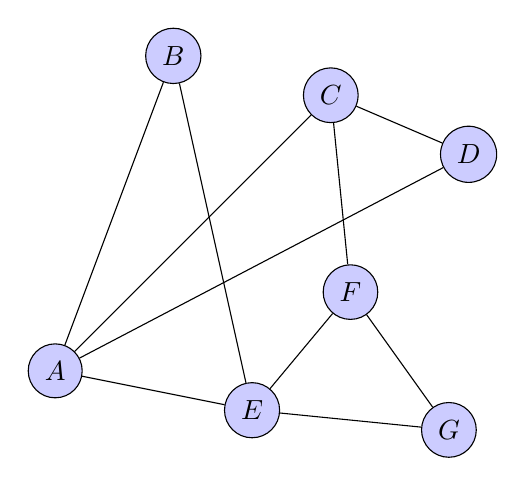
\begin{tikzpicture}
           [dot/.style = {draw,fill=blue!20,circle}]
            \node[dot] (B) at (-0.5, 0) {$B$};
            \node[dot] (C) at (1.5,-0.5) {$C$};
            \node[dot] (D) at (3.25,-1.25) {$D$};
            \node[dot] (A) at (-2,-4) {$A$};
            \node[dot] (F) at (1.75,-3) {$F$};
            \node[dot] (E) at (0.5,-4.5) {$E$};
            \node[dot] (G) at (3,-4.75) {$G$};
        
            \path[-] (A) edge (B);
            \path[-] (A) edge (C);
            \path[-] (A) edge (D);
            \path[-] (A) edge (E);
            \path[-] (B) edge (E);
            \path[-] (C) edge (F);
            \path[-] (C) edge (D);
            \path[-] (F) edge (E);
            \path[-] (F) edge(G);
            \path[-] (G) edge (E);
        \end{tikzpicture}
    \end{center}
    \begin{itemize}
        \item[a)] What is the degree of node E?

        4
        
        \item[b)] List two paths from A to D, and their corresponding length (there are more than 3).

        A$\,\to\,$D, Length: 1\\
        A$\,\to\,$B$\,\to\,$E$\,\to\,$F$\,\to\,$C$\,\to\,$D, Length: 5        
        \item[c)] List a cycle in the graph, and its corresponding length.

        A$\,\to\,$C$\,\to\,$F$\,\to\,$E$\,\to\,$A, Length: 4
        
        \item[d)] Show the adjacency matrix of the graph.

        $
        \begin{matrix}
         & A & B & C & D & E & F & G \\
         A & 0 & 1 & 1 & 1 & 1 & 0 & 0 \\
         B & 1 & 0 & 0 & 0 & 1 & 0 & 0 \\
         C & 1 & 0 & 0 & 1 & 0 & 1 & 0 \\
         D & 1 & 0 & 1 & 0 & 0 & 0 & 0 \\
         E & 1 & 1 & 0 & 0 & 0 & 1 & 1 \\
         F & 0 & 0 & 1 & 0 & 1 & 0 & 1 \\
         G & 0 & 0 & 0 & 0 & 1 & 1 & 0 
        \end{matrix}
        $
        
        \newpage
        
        \item[e)] Show the adjacency list of the graph.

        \begin{center}
            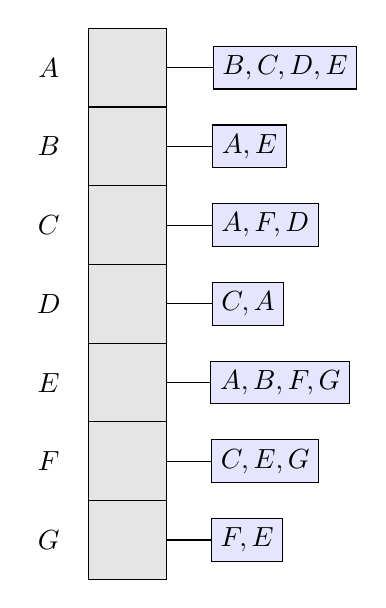
\begin{tikzpicture}
                [dot/.style = {minimum size = 1cm, draw, fill=gray!20}, dot1/.style={minimum size = 0.5cm, draw, fill=blue!10}]
                % Index in has table
                \node  (A) at (-1,0) {$A$};
                \node  (B) at (-1,-1) {$B$};
                \node  (C) at (-1,-2) {$C$};
                \node  (D) at (-1,-3) {$D$};
                \node  (E) at (-1,-4) {$E$};
                \node  (F) at (-1,-5) {$F$};
                \node  (G) at (-1,-6) {$G$};
                % Nodes representing spots in memory at corresponding index
                \node[dot] (a) at (0, 0) {};
                \node[dot] (b) at (0,-1) {};
                \node[dot] (c) at (0,-2) {};
                \node[dot] (d) at (0,-3) {};
                \node[dot] (e) at (0,-4) {};
                \node[dot] (f) at (0,-5) {};
                \node[dot] (g) at (0,-6) {};

                % Chains
                \node[dot1] (aa) at (2,0) {$B, C, D, E$};
                \node[dot1] (bb) at (1.55,-1) {$A, E$};
                \node[dot1] (cc) at (1.75,-2) {$A, F, D$};
                \node[dot1] (dd) at (1.53,-3) {$C, A$};
                \node[dot1] (ee) at (1.94,-4) {$A, B, F, G$};
                \node[dot1] (ff) at (1.75,-5) {$C, E, G$};
                \node[dot1] (gg) at (1.52,-6) {$F, E$};
                % Lines
                \path[-] (a) edge (aa);
                \path[-] (b) edge (bb);
                \path[-] (c) edge (cc);
                \path[-] (d) edge (dd);
                \path[-] (e) edge (ee);
                \path[-] (f) edge (ff);
                \path[-] (g) edge (gg);
            \end{tikzpicture}
        \end{center}
        
        \item[f)] Show the order of nodes visited with \textbf{breath first search} algorithm, starting with vertex A.

        Order of visited was determined when the node was dequeued: 

        A$\,\to\,$B$\,\to\,$C$\,\to\,$D$\,\to\,$E$\,\to\,$F$\,\to\,$G

        \begin{centering}
            \begin{tabular}{|c|c|c|}
                \hline
                \emph{v} & edge to & dist to\\
                \hline
                A & - & 0\\
                \hline
                B & A & 1\\
                \hline
                C & A & 1\\
                \hline
                D & A & 1\\
                \hline
                E & A & 1\\
                \hline
                F & C & 2\\
                \hline
                G & E & 2\\
                \hline
            \end{tabular}
        \end{centering}
        
        \item[g)] Show the order of nodes visited with \textbf{depth first search} algorithm, starting with vertex A.

        Order of visited nodes was determined when the node was first visited(inorder).  The largest node adjacent to current node was selected to travel to next: 

        A$\,\to\,$E$\,\to\,$G$\,\to\,$F$\,\to\,$C$\,\to\,$D$\,\to\,$B

        \begin{centering}
            \begin{tabular}{|c|c|c|}
                \hline
                \emph{v} & marked & edge to\\
                \hline
                A & T & -\\
                \hline
                B & T & E\\
                \hline
                C & T & F\\
                \hline
                D & T & C\\
                \hline
                E & T & A\\
                \hline
                F & T & G\\
                \hline
                G & T & E\\
                \hline
            \end{tabular}
        \end{centering}
        
    \end{itemize}
\end{itemize}

\end{document}
